%Chapter 5 - Current state of the MEGA65 project
%What is the current state of the MEGA65 project?

\chapter{Current state of the MEGA65 project as of March, 2019}
\label{cha: Chapter5}
This chapter discusses the current state of the MEGA65 project in both its form-factors. 
%----------------------------------------------------------------------------------------
%----------------------------------------------------------------------------------------
\section{MEGAphone}
This section looks at the current state of the MEGAphone. The MEGAphone is the hand-held console form-factor of the MEGA65. 

\subsection{Hardware}
The MEGAphone electronics hardware is currently in an alpha stage, the PCB is in its first revision and is mostly populated with components but there is expected to be faults in the design. A picture of the PCB with and without components is shown below in figure \ref{MEGAphone_PCB_r1_empty} and \ref{MEGAphone_PCB_r1_populated}. A visual inspection of the PCB and discussion with Dr Paul Gardner-Stephens led to the following lists of faults, things to be tested and other note-worthy decisions relating to the current state of the MEGAphone hardware. \\

\begin{figure} \begin{center}
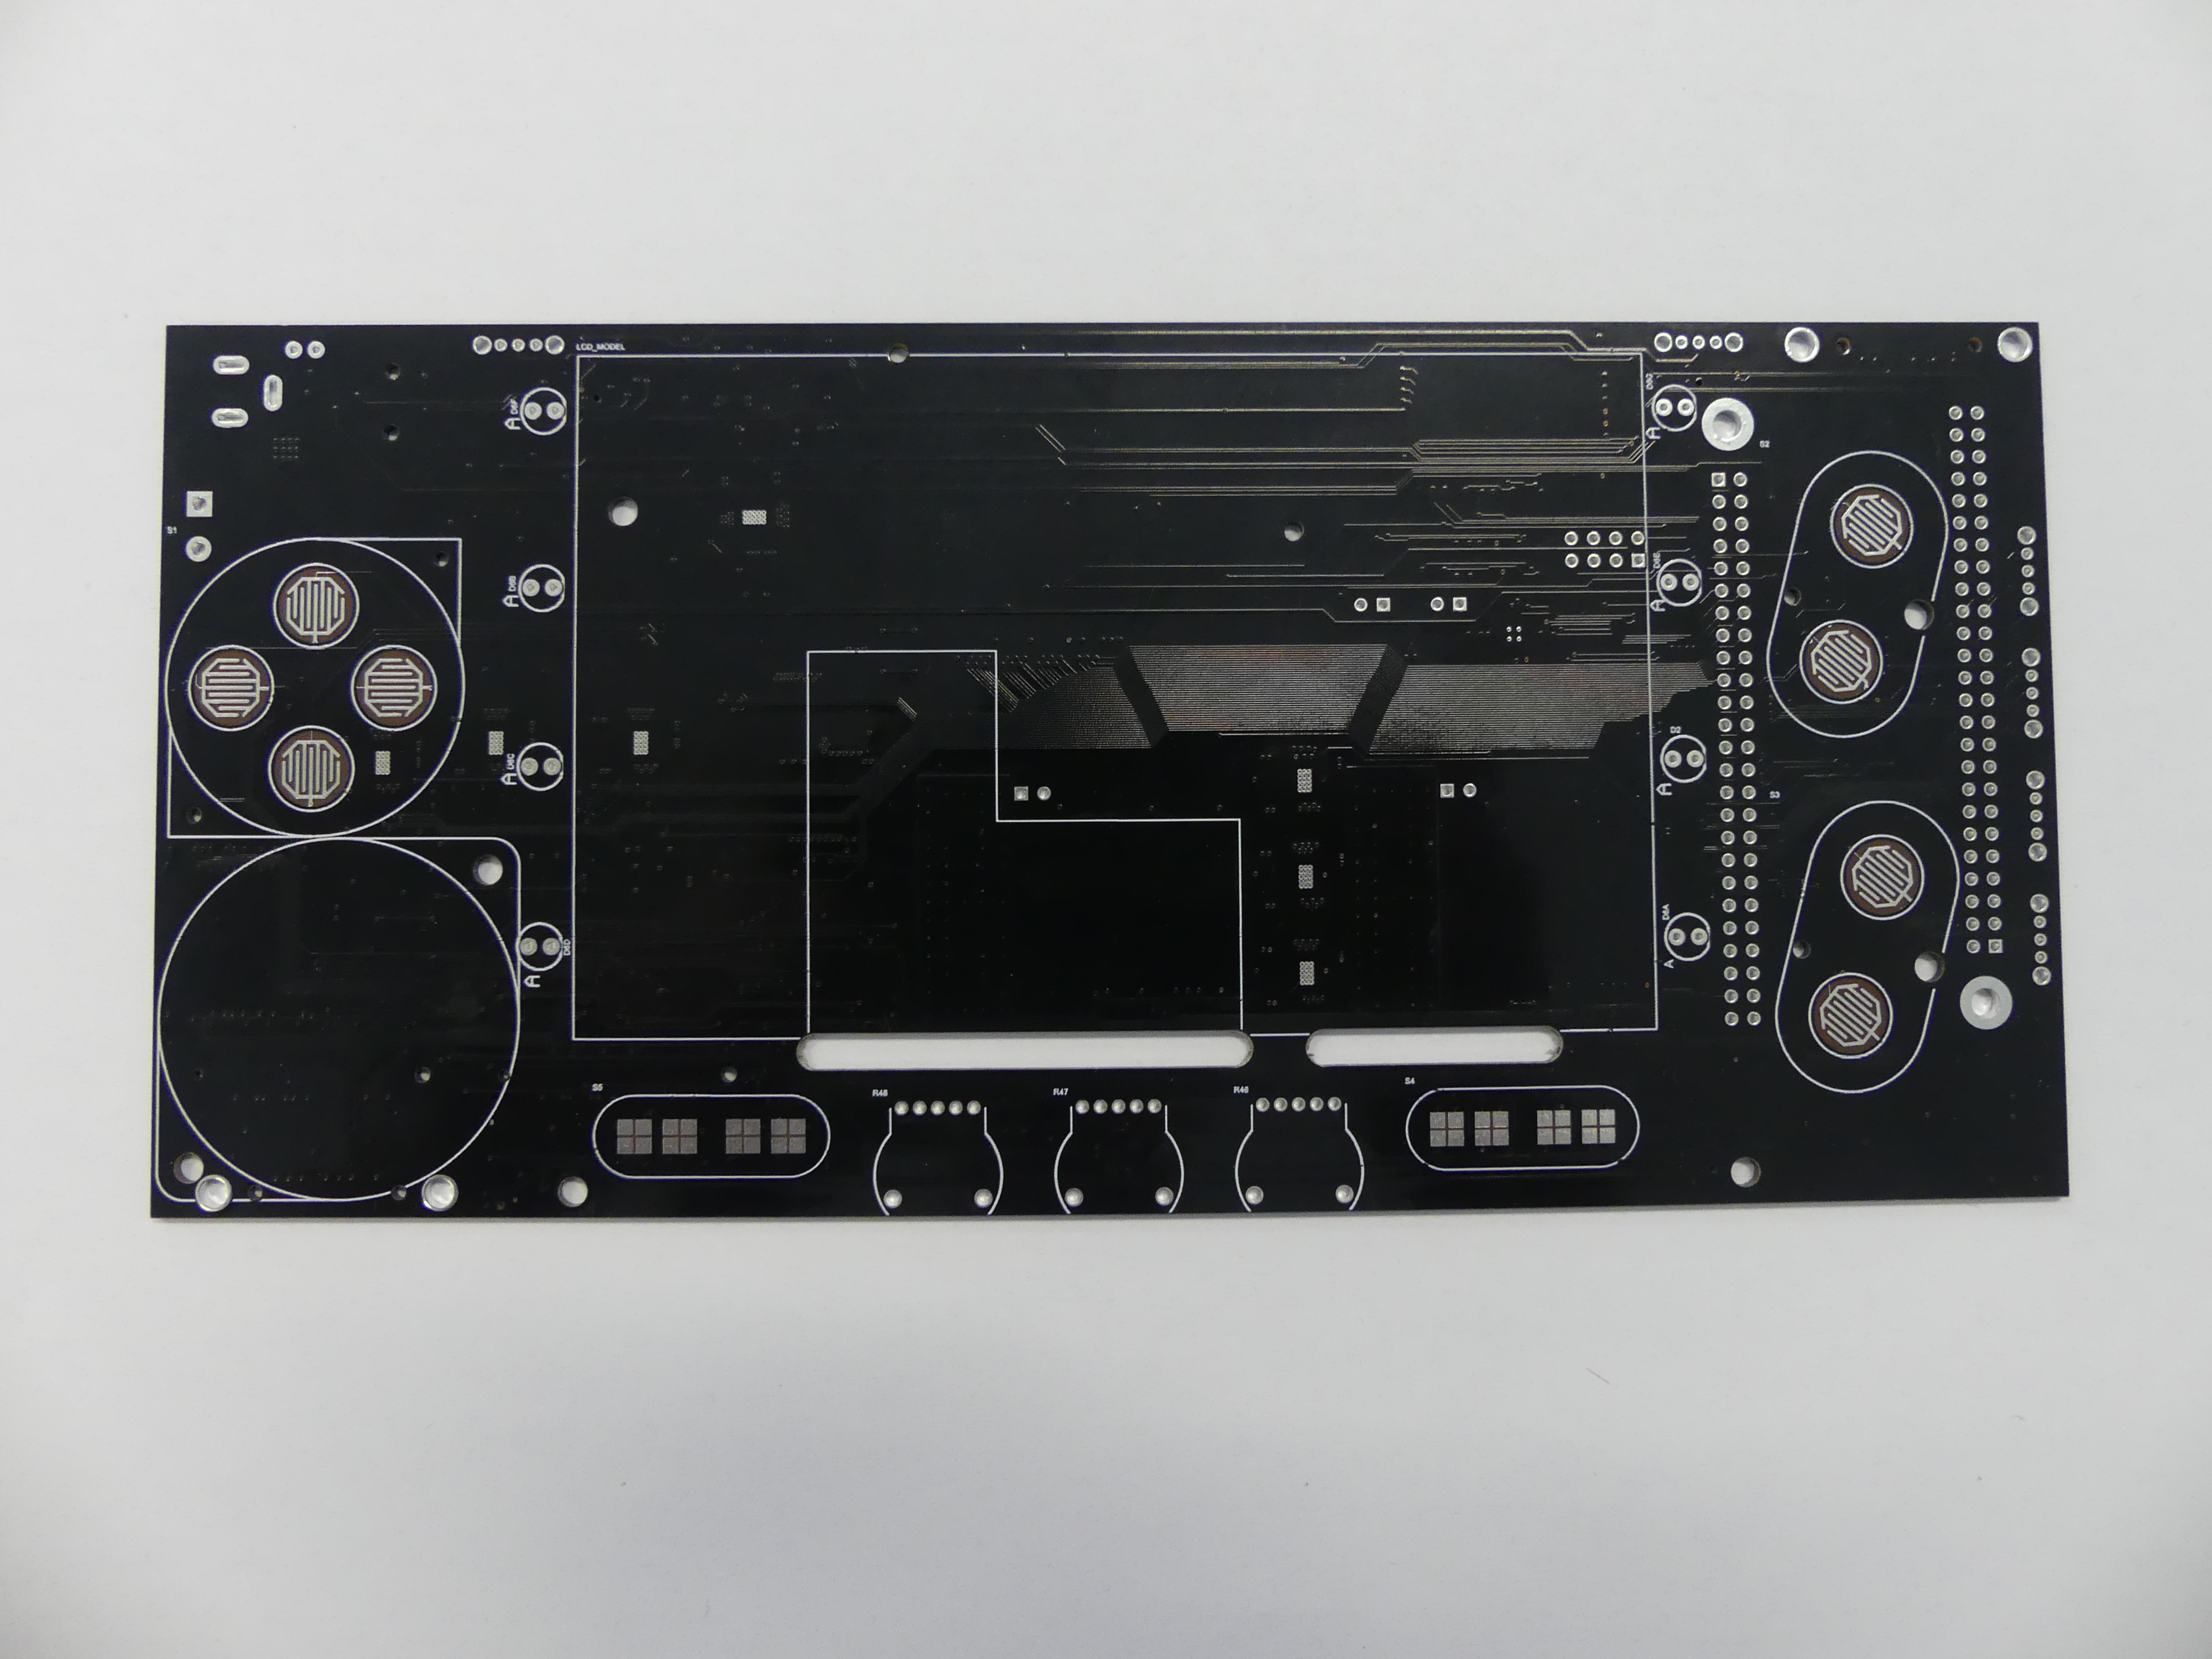
\includegraphics[width=.3\linewidth]{pics/MEGAphone_PCB_r1_empty_front} 
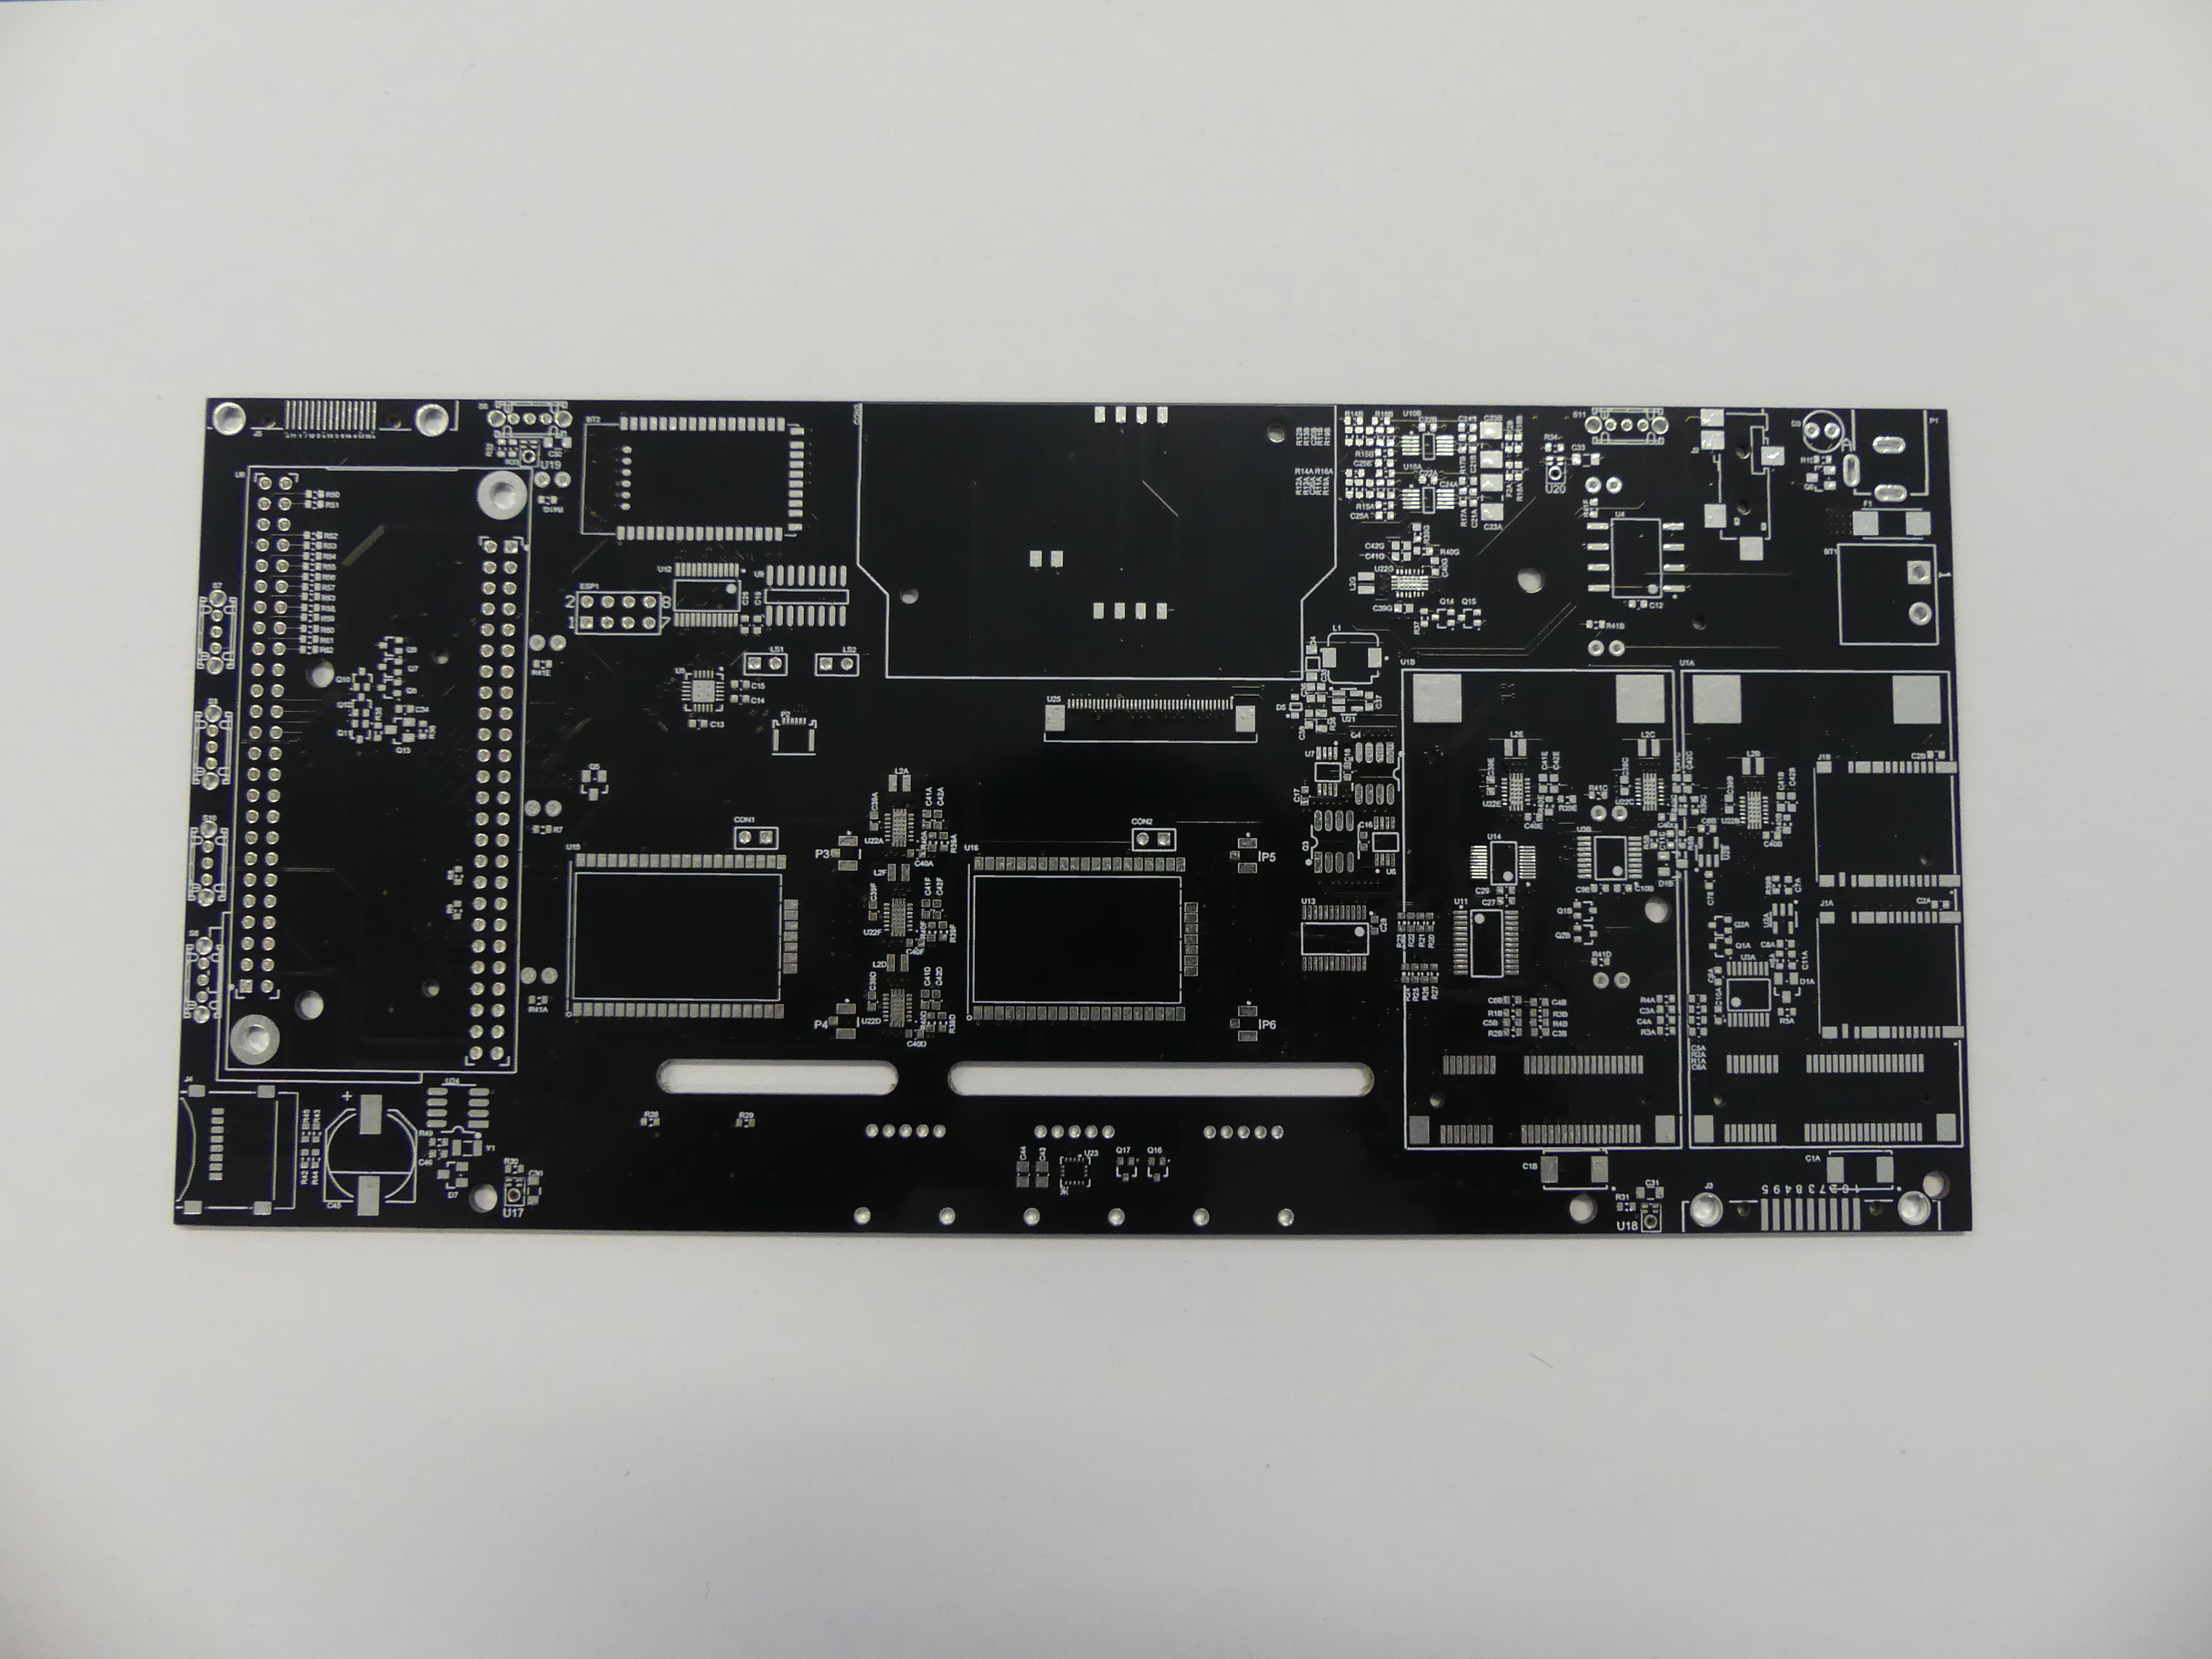
\includegraphics[width=.3\linewidth]{pics/MEGAphone_PCB_r1_empty_back} 
\end{center} 
\caption{MEGAphone PCB Revision 1 from the front and back when not populated with components. Front side is shown of the left.\\}
\label{MEGAphone_PCB_r1_empty}
\end{figure}

\begin{figure} \begin{center}
\includegraphics[width=.3\linewidth]{pics/MEGAphone_PCB_r1_populated_front} 
\includegraphics[width=.3\linewidth]{pics/MEGAphone_PCB_r1_populated_back} 
\end{center} 
\caption{MEGAphone PCB Revision 1 from the front and back populated with components. Front side is shown of the left.\\}
\label{MEGAphone_PCB_r1_populated}
\end{figure}


\textbf{Faults in Hardware}
\begin{enumerate}
\item The joystick connector, J3, is the wrong gender, currently it is female where as it should be male, figure \ref{MEGAphone_PCB_r1_J3}.
\item U1A and U1B, the footprint of the latch that holds the cellular modem is in the wrong position, figure \ref{MEGAphone_PCB_r1_U1A}.
\item U14 is not populated, this is the external joystick controller, figure \ref{MEGAphone_PCB_r1_U14}. 
\item U4 is currently missing, this is the Analogue-to-Digital converter for the microphone, figure \ref{MEGAphone_PCB_r1_U4}.
\item U25 needs to be moved a few millimetres to the right (when looking at the PCB face the component is mounted to) and also a couple of millimetres towards the slot which the ribbon runs through. This is to allow the ribbon cable to connect easier, figure \ref{MEGAphone_PCB_r1_U25}.
\item P2 need to be re-positioned a couple of millimetres towards the ribbon cable slot to allow the ribbon to connect easier \ref{MEGAphone_PCB_r1_P2}.
\item U15 may need to be moved a few millimetres to the left (when looking at the component) to allow for the ribbon cable to reach P2 without rubbing on U15 figure \ref{MEGAphone_PCB_r1_P2}.
\item LED power indicator are slightly too close together to allow the screen cover to fit between them \ref{MEGAphone_PCB_r1_LED}.
\item U9 which is the SPI flash chip, the footprint is wrong i.e. doesn't match the part, figure \ref{MEGAphone_PCB_r1_U9}.
\item R46, R47 and R48, the thumb wheels for volume control, are missing and currently on back order, figure \ref{MEGAphone_PCB_r1_R49_R48_R47}.
\item Found the PCB is outputting over 6.45 Volts where it should be outputting 3.3V. \\
\end{enumerate}

\begin{figure} \begin{center}
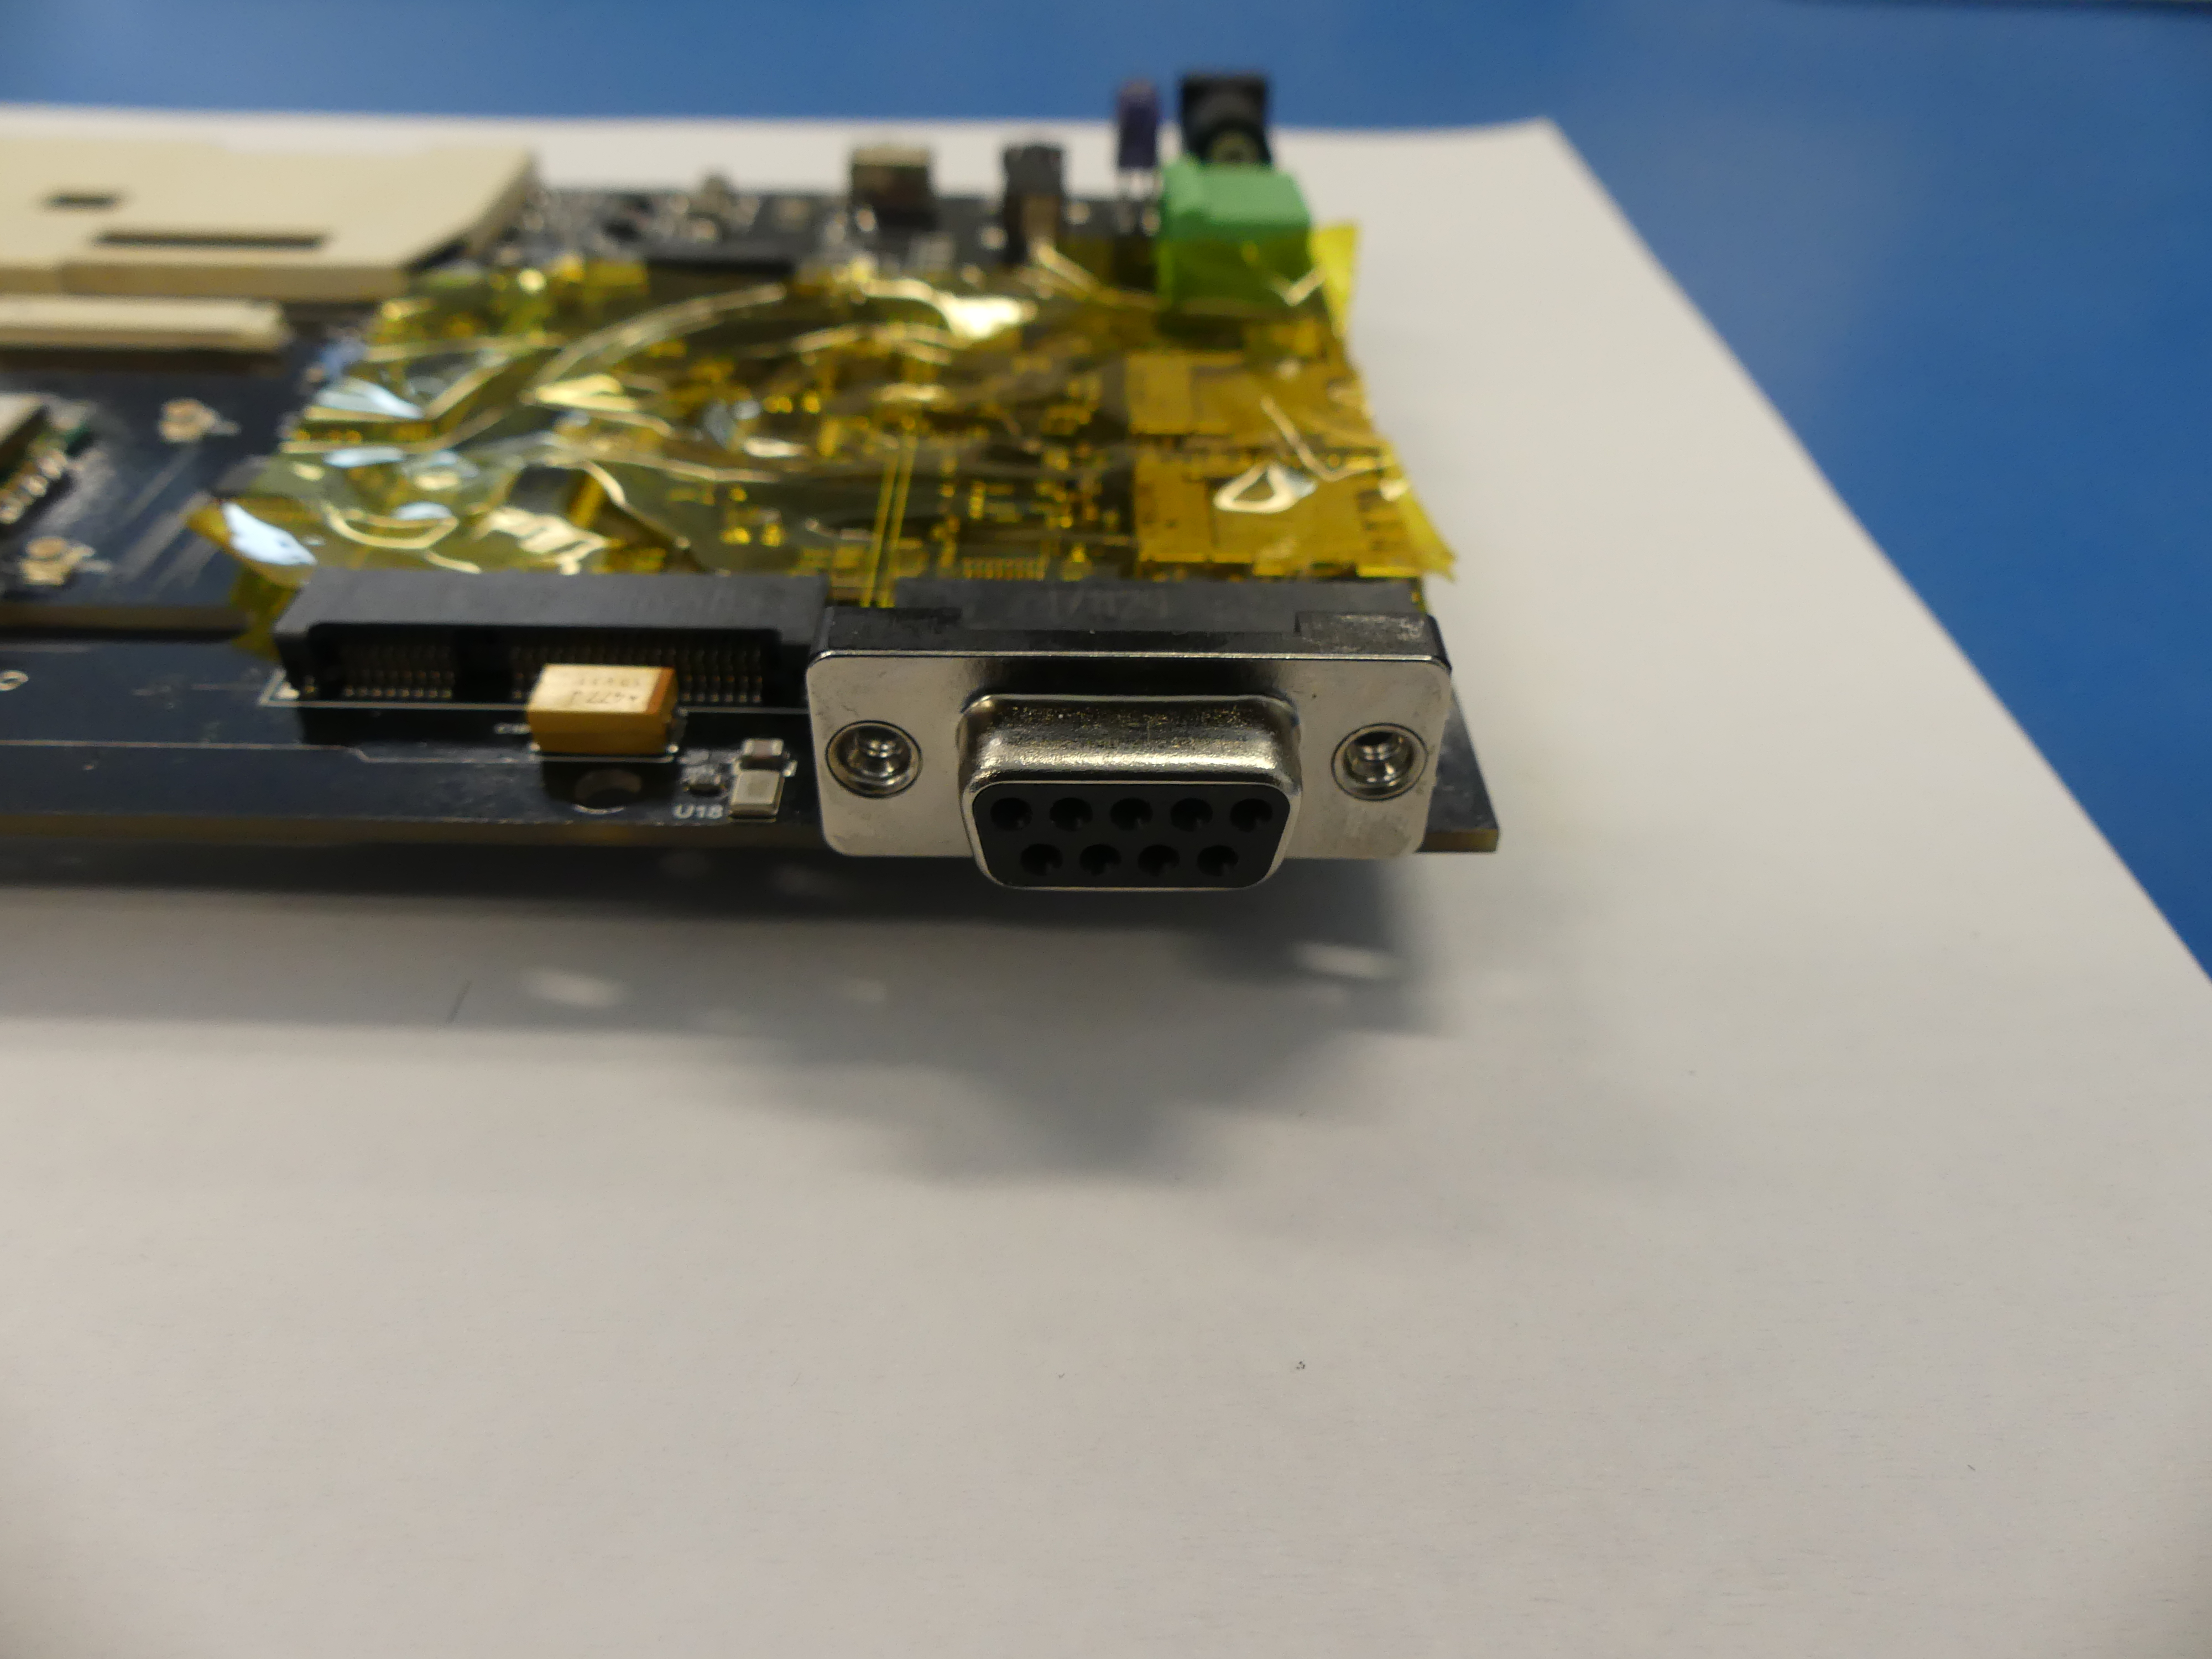
\includegraphics[width=.3\linewidth]{pics/MEGAphone_PCB_r1_J3} 
\end{center} 
\caption{Close up of Joystick connector J3, which should be a male connector.\\}
\label{MEGAphone_PCB_r1_J3}
\end{figure}

\begin{figure} \begin{center}
\includegraphics[width=.3\linewidth]{pics/MEGAphone_PCB_r1_U1A} 
\end{center} 
\caption{Close up showing the latch installed in U1B but not U1A.\\}
\label{MEGAphone_PCB_r1_U1A}
\end{figure}

\begin{figure} \begin{center}
\includegraphics[width=.3\linewidth]{pics/MEGAphone_PCB_r1_U14} 
\end{center} 
\caption{Close up showing unpopulated component U14.\\}
\label{MEGAphone_PCB_r1_U14}
\end{figure}

\begin{figure} \begin{center}
\includegraphics[width=.3\linewidth]{pics/MEGAphone_PCB_r1_U4} 
\end{center} 
\caption{Close up showing unpopulated component U4.\\}
\label{MEGAphone_PCB_r1_U4}
\end{figure}

\begin{figure} \begin{center}
\includegraphics[width=.3\linewidth]{pics/MEGAphone_PCB_r1_U25}
\includegraphics[width=.3\linewidth]{pics/MEGAphone_PCB_r1_U25_P2_ribbon}
\end{center} 
\caption{Close up showing component U25 as well with as the ribbon connector for the screen. U25 needs to be re-positioned.\\}
\label{MEGAphone_PCB_r1_U25}
\end{figure}

\begin{figure} \begin{center}
\includegraphics[width=.3\linewidth]{pics/MEGAphone_PCB_r1_P2}
\includegraphics[width=.3\linewidth]{pics/MEGAphone_PCB_r1_U25_P2_ribbon}
\end{center} 
\caption{Close up showing component P2 as well with as the ribbon connector for the screen. P2 needs to be re-positioned. \\}
\label{MEGAphone_PCB_r1_P2}
\end{figure}

\begin{figure} \begin{center}
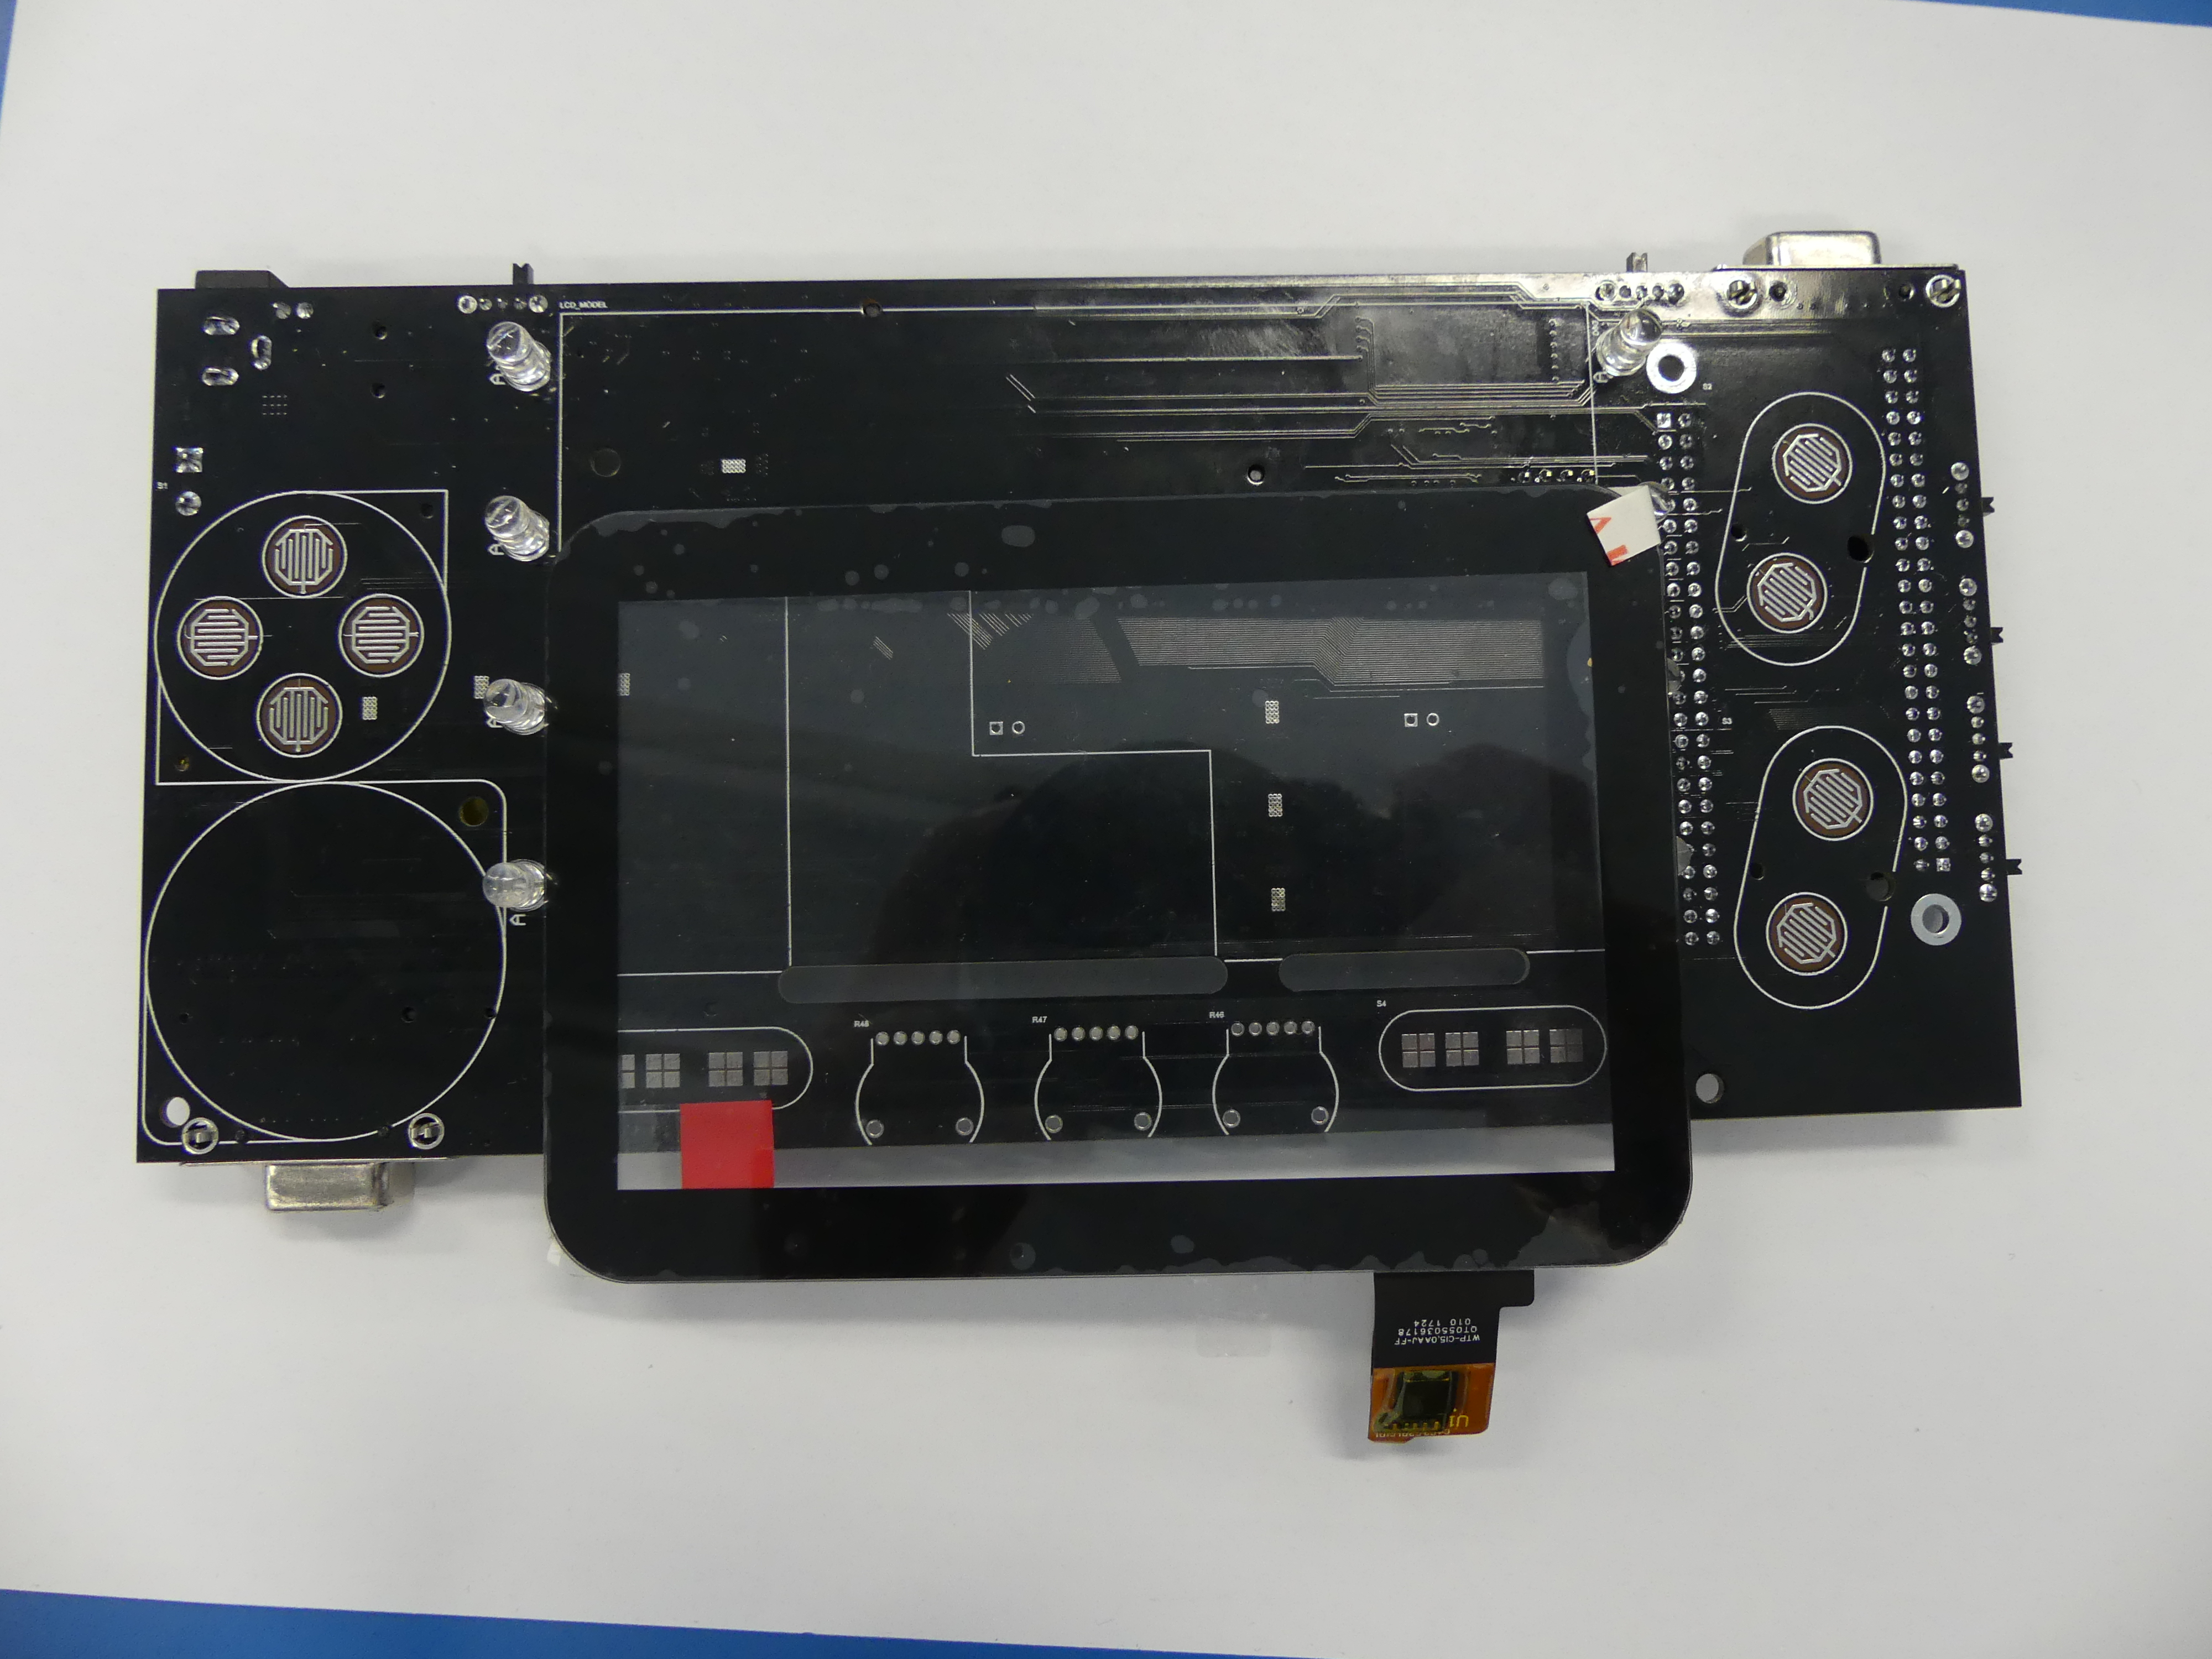
\includegraphics[width=.3\linewidth]{pics/MEGAphone_PCB_r1_LED1}
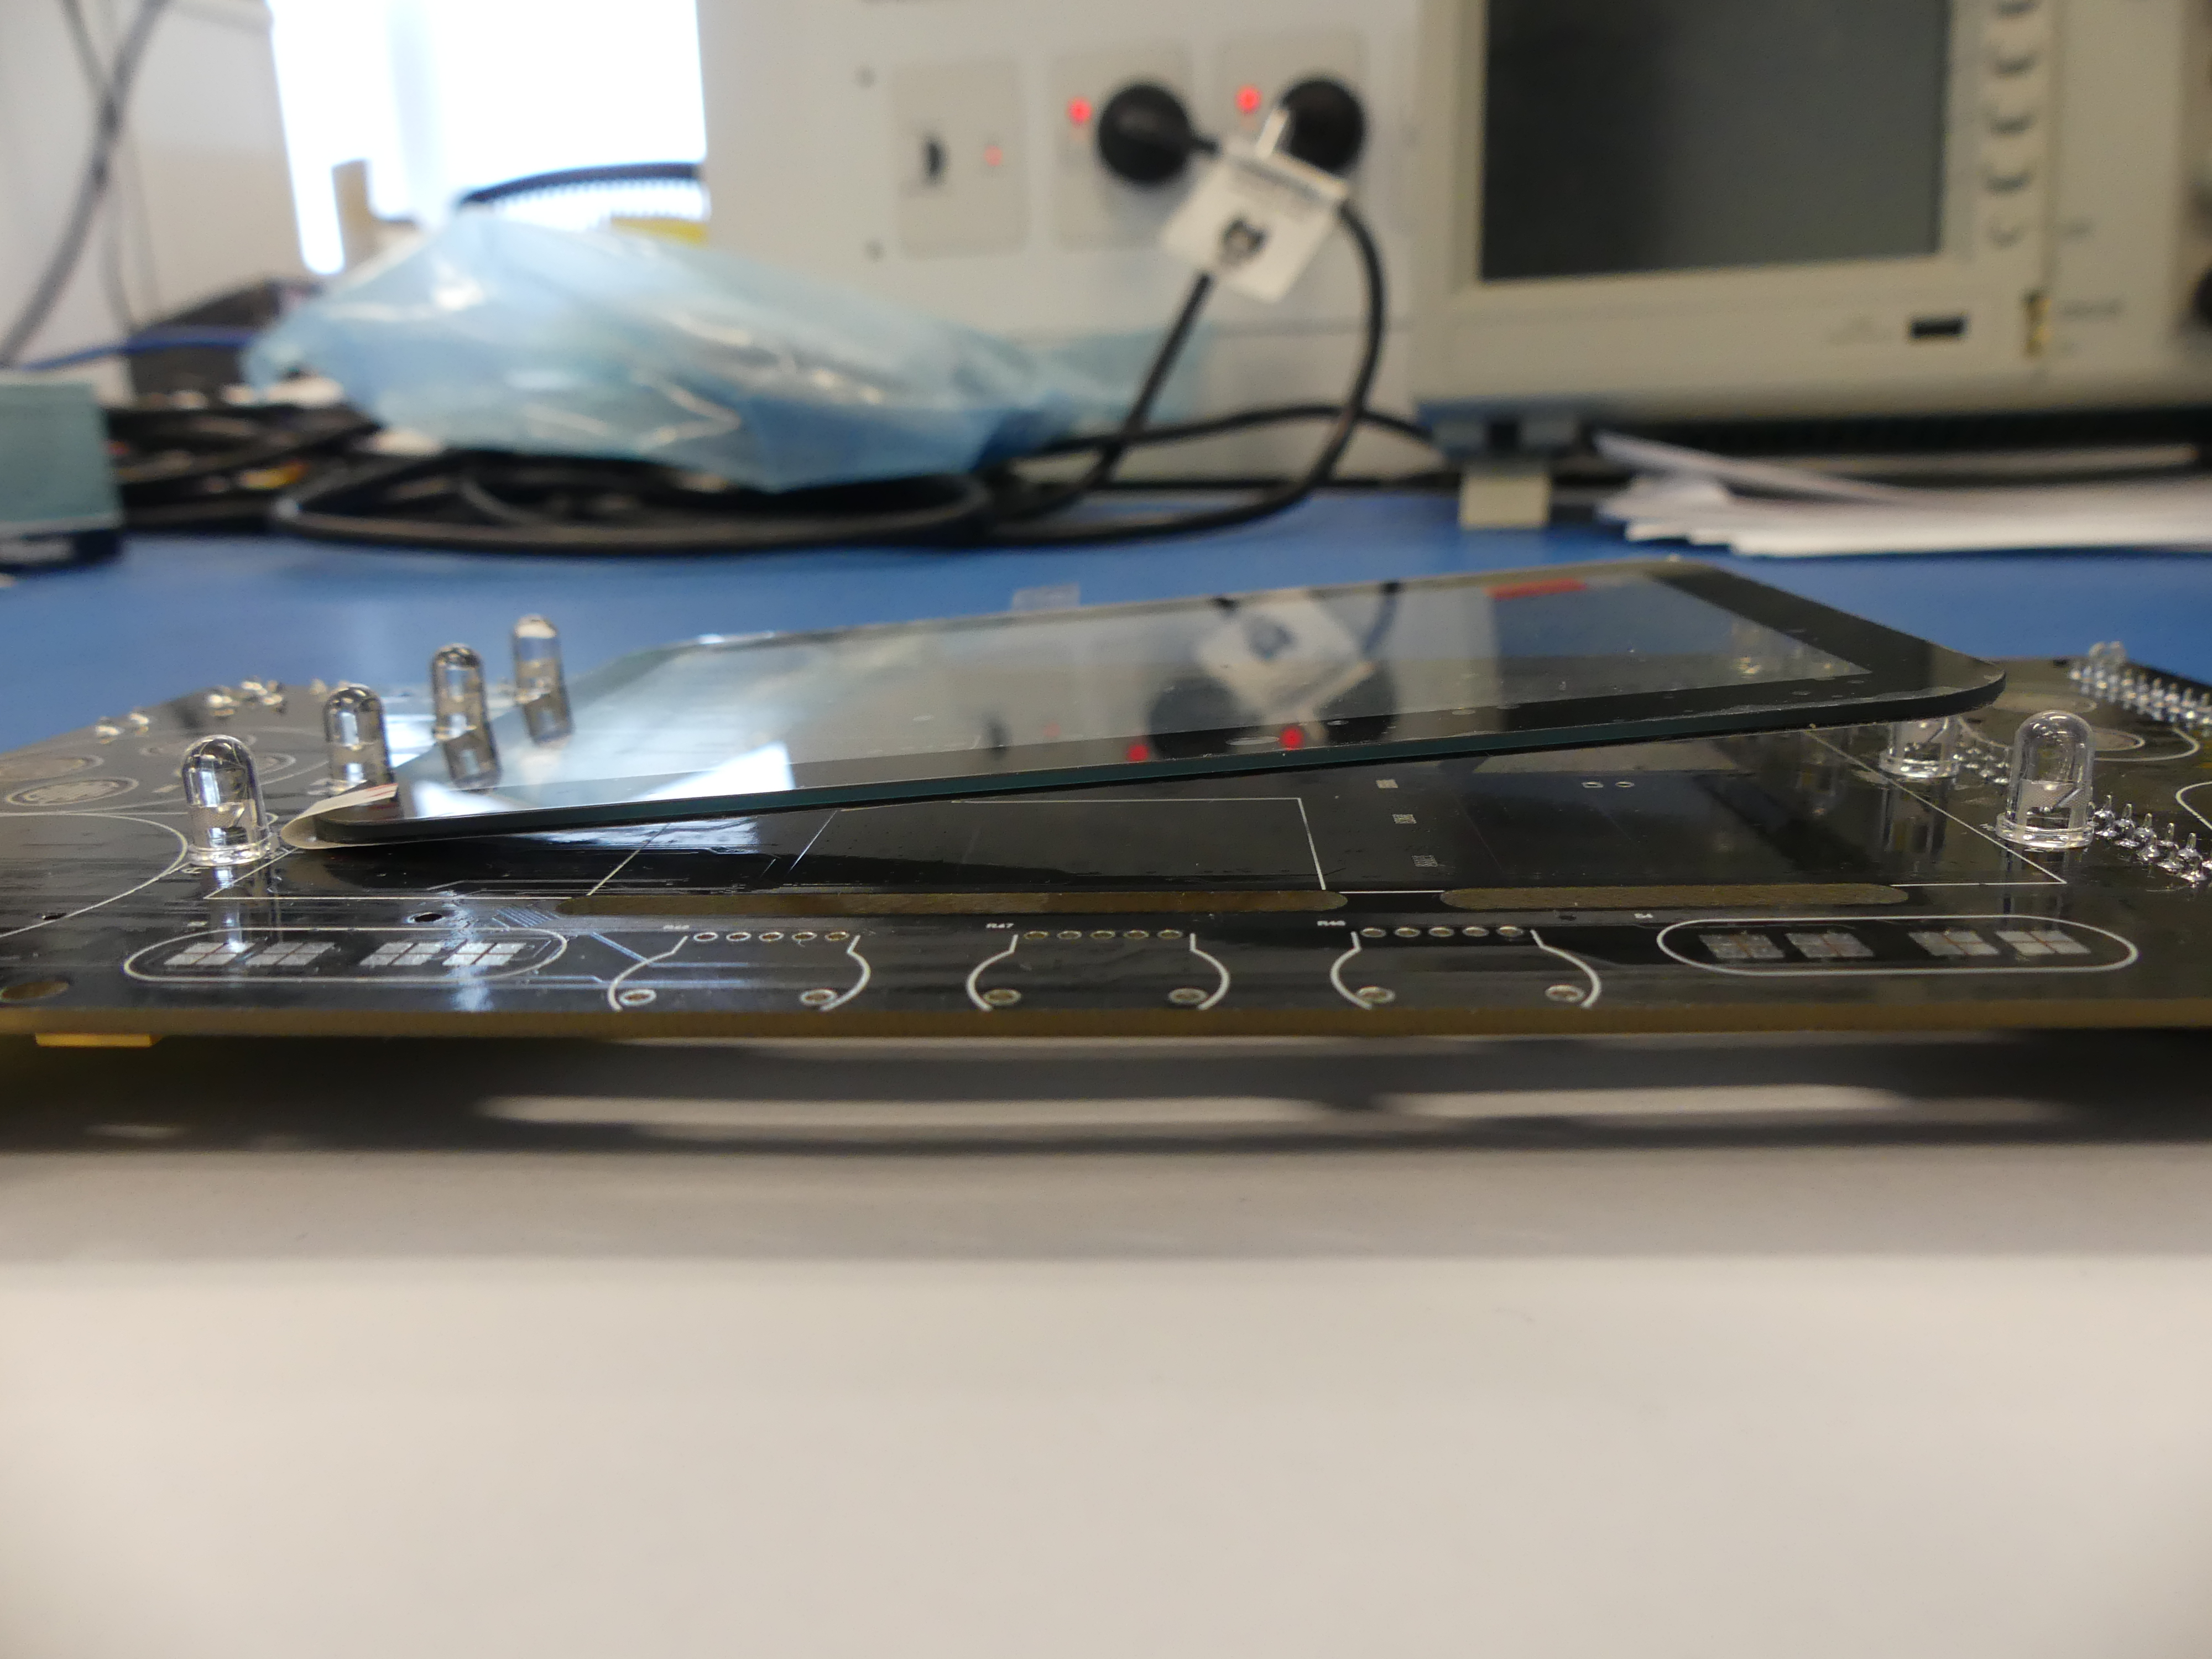
\includegraphics[width=.3\linewidth]{pics/MEGAphone_PCB_r1_LED2}
\includegraphics[width=.3\linewidth]{pics/MEGAphone_PCB_r1_LED3}
\end{center} 
\caption{Close up showing position of LED on front face of PCB. Screen cannot fit between them. \\}
\label{MEGAphone_PCB_r1_LED}
\end{figure}

\begin{figure} \begin{center}
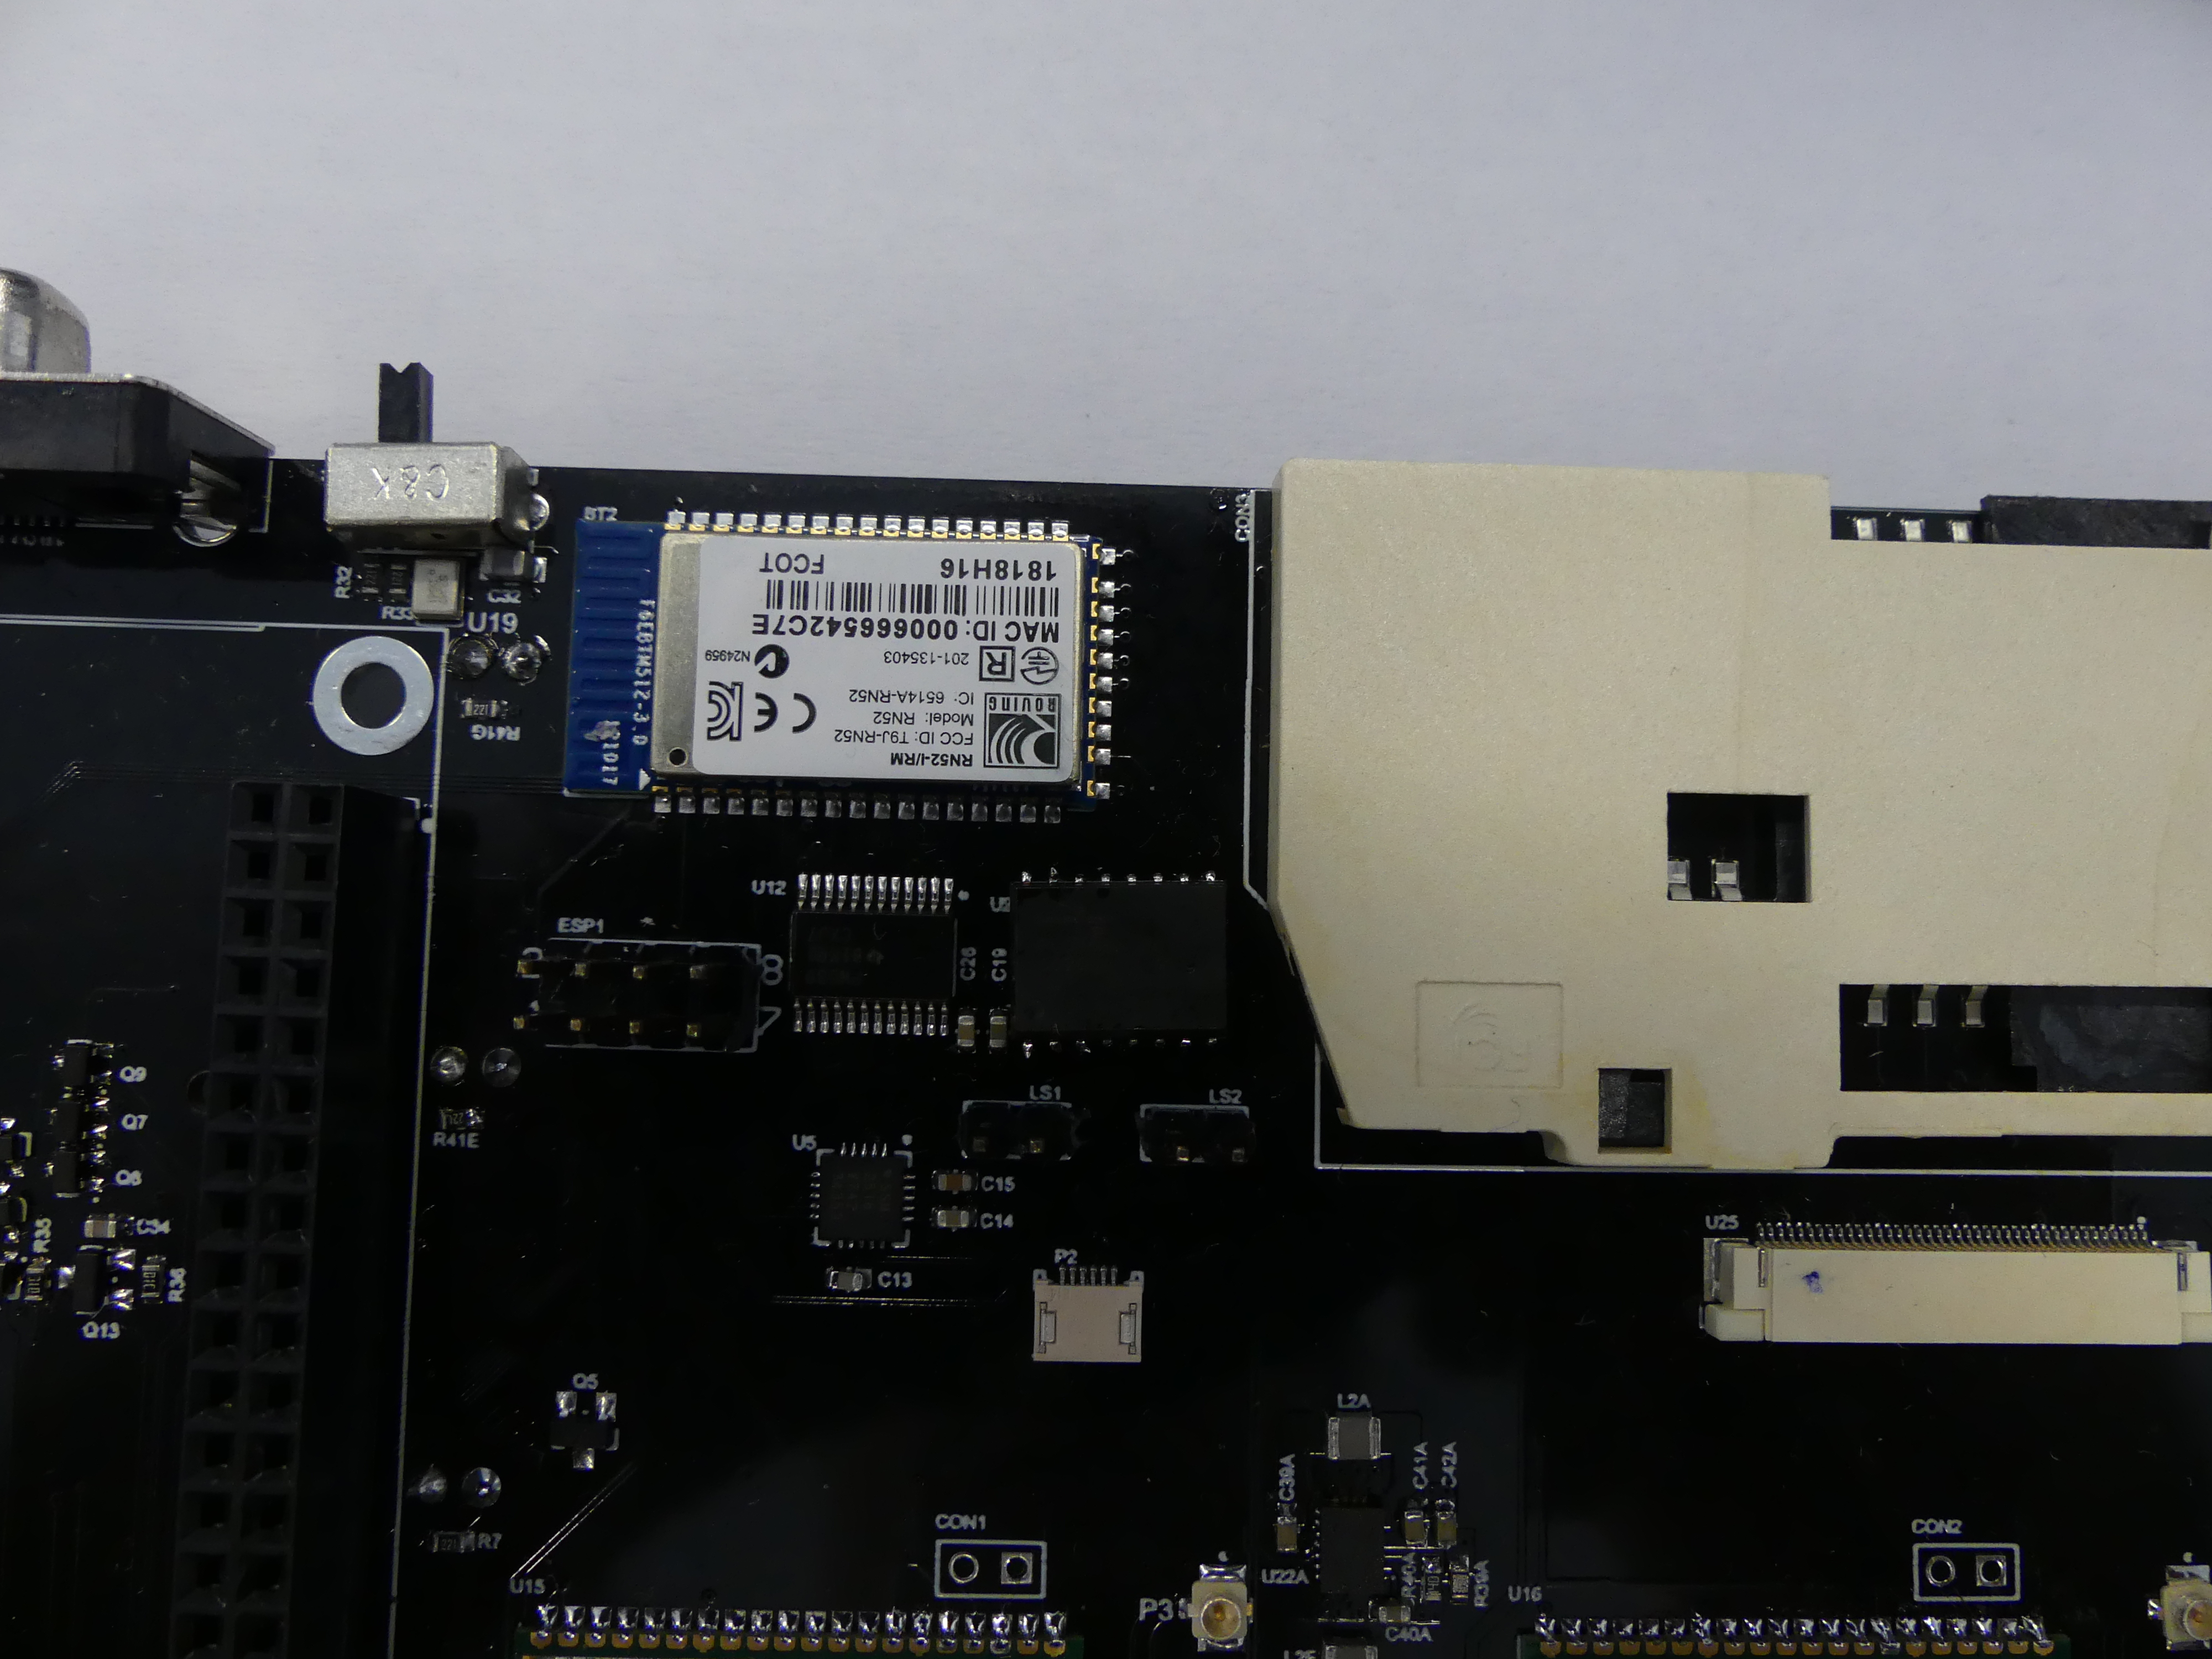
\includegraphics[width=.3\linewidth]{pics/MEGAphone_PCB_r1_U9}
\end{center} 
\caption{Close up of U9 which didn't fit its footprint and had to be modified to fit. \\}
\label{MEGAphone_PCB_r1_U9}
\end{figure}

\begin{figure} \begin{center}
\includegraphics[width=.3\linewidth]{pics/MEGAphone_PCB_r1_R48_R47_R46}
\includegraphics[width=.3\linewidth]{pics/MEGAphone_PCB_r1_populated_front}
\end{center} 
\caption{Close up of missing thumb wheels for volume control, R46, R47 and R48. \\}
\label{MEGAphone_PCB_r1_R49_R48_R47}
\end{figure}

\textbf{Things that need to be tested}
\begin{enumerate}
\item U1A and U1B, might not have enough clearance to fit the cellular modems in place due to components mounted on PCB in this area. 4G modem component to be used to test if it fits. Components within U1A and U1B footprint may need to be relocated if the 4G modem doesn't fit. In particular, the components J1A and J1B may need to be lower profile connectors such as a SIM card connector without the microSD slot above it, which it currently has on both J1A and J1B. Shown in figure \ref{MEGAphone_PCB_r1_U1A_clearance} \\
\end{enumerate}

\begin{figure} \begin{center}
\includegraphics[width=.3\linewidth]{pics/MEGAphone_PCB_r1_U1A_clearance1}
\includegraphics[width=.3\linewidth]{pics/MEGAphone_PCB_r1_U1A_clearance2}
\end{center} 
\caption{Close up of clearance above U1A and U1B footprints, a cellular modem needs to be inserted in this space. \\}
\label{MEGAphone_PCB_r1_U1A_clearance}
\end{figure}


\textbf{Components or functions which cannot be tested currently}
\begin{enumerate}
\item Microphone audio.
\item Thumb wheels for volume control, R48, R47 and R46.
\item 2nd PCIe modem slot, U1A.
\item 2nd SIM card slot, associated with the 2nd modem, U1A, mentioned above.
\item The ribbon cable connections between U25, P2 and the screen cannot be fully tested with the screen in position but a partial test with the screen offset should be possible.
\item Speaker currently not installed but parts and component are present in lab. \\
\end{enumerate}

\textbf{Noteworthy feature}
\begin{enumerate}
\item Installation of insulating tape covering components within the U1A and U1B footprints. This is to provide insulation between conductive part of components and the modem which will be inserted above them. \\
\end{enumerate}


\subsection{Software}



%----------------------------------------------------------------------------------------
%----------------------------------------------------------------------------------------
\section{Desktop Computer Form Factor}
